\documentclass{article}
\usepackage{graphicx} % Required for inserting images

\usepackage[french]{babel}
\usepackage[T1]{fontenc}
\usepackage{lmodern}
\usepackage{hyperref}
\usepackage{wrapfig}

\title{Rapport de projet : Chat201 – édition thread \& réseau}
\author{Daniel DEFOING (\texttt{ddef0003}) \and 
        Belinda ÖZNUR (\texttt{bozn0003}) \and
        Haluk YILMAZ (\texttt{hyil0003})}
\date{\today}

\begin{document}
\pagenumbering{gobble}

\maketitle
\tableofcontents
\newpage

\pagenumbering{arabic}
\section{Introduction}
Ce rapport décrit globalement la conception du second projet dans le cadre du cours de Systèmes d'Exploitation
(INFO-F201). Il présente les choix de conception qui ont guidé notre développement, et les difficultés qui ont pu survenir durant celui-ci. Pour voir de façon précise les changements ayant eu lieu tout au long du projet et la contribution de chacun, veuillez consulter \hyperref[https://github.com/Daniel-Dfg/OS_Projet_2]{le repository GitHub de notre projet}.

\section{Choix du langage :pourquoi C++ plutôt que C ?}

\subsection*{Des outils qui facilitent le développement en général}
Une raison fondamentale qui a guidé cette décision est que C++ possède des fonctionnalités absentes en C tels que les références, les chaînes de caractères (ou \textit{strings}, qu'on a souvent subsitués aux \texttt{char*[]}) ou encore les classes. 

On peut aussi parler des conteneurs STL comme \texttt{std::vector} ou \texttt{std::queue}, très utilisés dans cette implémentation du projet.

Or, dans le cadre du projet présenté ici, ces éléments apportent une pluvalue non négligeable en permettant de structurer un code de façon plus fine qu'en C ou de simplifier grandement certaines opérations. L'exemple le plus trivial qu'on peut donner de ceci est le passage de paramètres par référence plutôt que par pointeur dans certaines fonctions, qui permet une gestion plus sûre de la mémoire.

\subsection*{Des librairies qui fournissent des abstractions utiles pour ce projet}
On va illustrer ce point en parlant des \textit{threads}. En langage C, on utilisera \texttt{thread.h} pour les gérer, alors qu'en C++ on a par exemple accès à la librarie \texttt{std::thread}, qui permet d'abstraire certaines opérations de la librarie en C (par exemple, accéder au thread courant avec \texttt{std::this\_thread}).

Utiliser C++ permet donc l'usage de certaines libraries standard absentes en C qui permettent d'abstraire des opérations de libraries \textit{correspondantes} en C.

\subsection*{Pas de perte notable à ne pas utiliser le langage C}
C++ reste évidemment compatible avec C : il n'existe pas d'opération en C infaisable exactement de la même façon en C++.
De plus, les deux langages étant connus pour leur rapidité d'exécution, la performance du C++ n'est pas dégradée de façon significative par rapport au C dans le cadre de ce projet.

L'utiliser permet donc de tirer parti ses abstractions discutées plus haut (voir 2 sections précédentes) tout en gardant une très bonne efficacité.


Tout ceci montre que les avantages majeurs ont été trouvés à utiliser C++ plutôt que C, alors qu’aucun avantage n’a été identifié en faveur de l’utilisation de C par rapport à C++. Ce choix du langage s’est donc naturellement imposé comme le plus adapté.

\section{Visualisation de l'architecture du programme}
Cette section discute des choix de conception du programme final, des considérations qui permettront au lecteur de mieux comprendre la nature de ces choix et des problèmes rencontrés qui en ont suivi.

\subsection{Le serveur en tant que \textit{point relais} des clients}
La structure d'un programme client-serveur tel que celui présenté ici peut être visualisée très simplement sous la forme d'un Graphe Étoile \cite{Graphe Étoile}, avec le serveur au centre et les clients aux extrémités de chaque branche. 
\begin{figure}[ht]
    \centering
    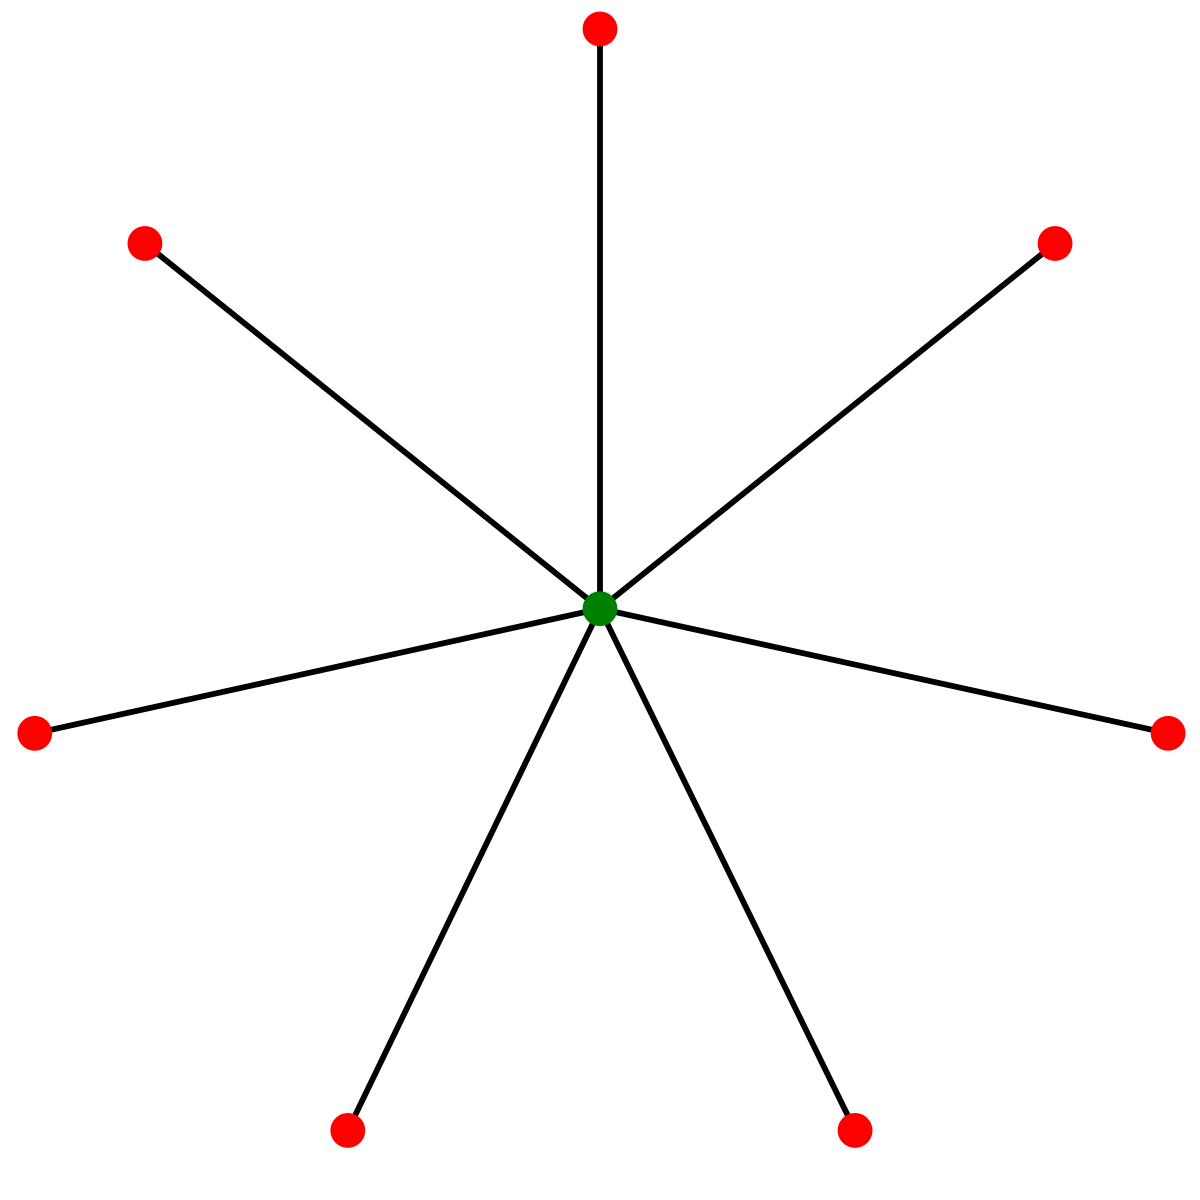
\includegraphics[width=0.25\linewidth]{etoile.png}
    \caption{\textit{Graphe Étoile typique.}}
\end{figure}

Cette représentation montre bien qu'un seul serveur se charge de \textit{relayer} les informations à passer d'un client à un autre ou d'un client vers lui-même (confirmation de (dé)connexion notamment). 

TODO : discuter du TCP/IP brièvement

Dans la suite, nous discuterons en profondeur de la façon dont les nœuds de ce graphe communiquent.

\subsection{Choix d'implémentation communs aux clients et au serveur}

\subsubsection{Deux \texttt{std::queue} (ou \textit{FIFOs}) à vider en permanence}
Tout client et le serveur ont chacun deux \texttt{std::queue} qu'ils observent en permanence: une pour les messages qu'ils envoient, et une pour celle qu'ils reçoivent. 

Utilser des \texttt{std::queue} n'ayant pas de taille limitée ainsi est une partie de la solution aux problèmes de synchronisation qui peuvent être rencontrés dans le cadre de ce projet. On va le montrer par deux exemples.


\textbf{Exemple 1 : un client reçoit plusieurs messages en même temps}

Dans le cas de l'implémentation choisie pour ce projet avec des FIFOs, les messages peuvent être \textit{push} à l'arrière de la FIFO servant et traités séquentiellement par le client qui la videra progressivement.


\textbf{Exemple 2 : Le serveur doit transmettre plusieurs messages à un même client}

Dans l'exemple 1, on a juste dit que les messages entraient dans une FIFO étaient vérifiés séquentiellement. Mais n'y a-t-il pas un risque que, si on envoie plusieurs messages simultanément à un même client, les deux messages risquent de corrompre la FIFO de réception du client (qui est un objet critique) en voulant s'insérer dedans en même temps ?


En principe, oui, c'est un problème qui peut survenir si on ne prend pas de précaution contre lui. Cependant, un bénéfice de notre implémentation avec des FIFOs est que, le serveur ayant une FIFO de \textit{messages à envoyer} qu'il vide progressivement, il garantit que les messages seront envoyés aux clients dans l'ordre où ils auront été reçus par le serveur, et on peut utiliser des mutex pour protéger la FIFO côté client (pour éviter qu'elle reçoive plusieurs messages simultanément).


Ces deux exemples ont illustré le fonctionnement des FIFOs de réception côté client et d'envoi côté serveur, mais la logique présentée s'applique symétriquement aux FIFOs d'envoi côté client et à la FIFO de réception côté serveur.

\subsubsection{De la méthode d'envoi des messages}
Il a été décidé d'abstraire l'échange d'informations entre les clients et le serveur principalement par une classe \texttt{Message}. Un point très important qui découle de ce choix d'implémentation est qu'on a utilisé des \texttt{std::string} pour garantir une gestion dynamique de la mémoire et simplifier les opérations de manipulation des chaînes de caractère.

\subsection{Conception des clients}

\subsubsection{Deux threads, deux FIFOs par client}
Ce point fait écho à la discussion sur l'usage de FIFOs côté client et serveur vue plus haut. 

Il faut préciser que le processus côté client se divise en deux \textit{threads}: un dédié à la réception des messages (qui doit donc vider et afficher le contenu de la FIFO de messages entrants) et un autre dédié à l'envoi de messages (qui doit donc en quelque sorte remplir la FIFO des messages à envoyer, puis la vider progressivement). 

Cette division du processus client en deux threads est due à des contraintes évidentes de performance et autorise le client à envoyer et recevoir des messages simultanément (gestion asynchrone des communications).

\subsubsection{Gestion de la (dé)connexion au serveur}
Tout client doit suivre le protocole TCP (réf. nécessaire) pour initialiser sa connexion et doit s'identifier auprès du serveur.
(incomplet)


 Gestion de la déconnexion (quel thread tue l'autre, comment on se déconnecte) TODO :
1. Signal de terminaison envoyé aux deux threads
2. Attente de la fin des opérations en cours
3. Libération des ressources
4. Fermeture propre de la connexion

\subsection{Conception du serveur}


TODO
\begin{itemize}
    \item Gestion des (dé)connexions
    \item Mapping des utilisateurs à leur file descriptors et inversement
    \item Gestion des sockets : surveillance permanente via \texttt{poll} (ou epoll le cas échéant)
    \item ...

\end{itemize}

\section{Améliorations non réalisées de l'implémentation actuelle}
\begin{itemize}
    \item Poll au lieu de epoll : "ouais ouais on aurait pu l'implémenter en quelques jours tkt"
    \item Attente active pour les FIFOs (on checke les queues en permanence plutôt que d'utiliser un système de notifications, un observer pattern (cf. cours de LDP2)).
\end{itemize}

\section{Difficultés rencontrées et solutions trouvées}
\subsection{Problèmes de synchronisation}
\begin{itemize}
    \item côté serveur, accès concurrents (problème producteur-consommateur)
    \item Signaux asynchrones (mentionner la conception du SignalManager dans l'explication de la solution)
    \item ...
\end{itemize}

\subsection{Garantie de l'intégrité du contenu partagé par les clients}
\begin{itemize}
    \item Gestion des tailles limites (longueur de pseudos et de messages)
    \item Comment s'est-on assurés que le messages étaient bien transmis sans perte ?
\end{itemize}


\begin{thebibliography}{999}
	\bibitem{Graphe Étoile}
		Wikipedia. (dernière modification : 2019, 21 janvier). \textit{Graphe étoile.} URL: \url{https://fr.wikipedia.org/wiki/Graphe_%C3%A9toile}, consulté le 12/12/2024.
\end{thebibliography}
\end{document}

